\pagebreak
\subsection{Metadata Performance}

As the \ac{RADOS} backend does not support the traditional file system layout required for mdtest, we have only performed metadata performance benchmarks using the \ac{CephFS} interface. The options shown in~\cref{tbl:mdtest-configured-options} were provided to mdtest for the performed benchmarks. Additionally, we provided the saveRankPerformanceDetails option to save the results to a file, which we parsed into our storage format as detailed in~\cref{sec:data-collection}.

\begin{table}[htbp]
\centering
\begin{tabular}{|lll|}
\hline
Flag               & Value & Description \\
\hline
\texttt{-n} & 16 & Number of files per task \\
\texttt{-U} & Enabled & Enable rename directory phase \\
\texttt{-R} & Enabled & Random file access \\
\texttt{-L} & Enabled & Files only at leaf level \\
\texttt{-C} & Enabled & Create files \\
\texttt{-T} & Enabled & Stat files \\
\texttt{-E} & Enabled & Read files \\
\texttt{-r} & Enabled & Remove files \\
\texttt{-u} & Enabled & Unique working directory per task \\
\texttt{-i} & 5 & Iteration count \\
\texttt{-w} & 4096 & Bytes to write to file after creation \\
\texttt{-e} & 4096 & Bytes to read from file after write \\
\texttt{-y} & Enabled & Sync file after writing \\
\texttt{-N} & 1 & Enable stride (reordering) for file operations \\
\texttt{-t} & Enabled & Time unique working directory overhead \\
\texttt{-{}-random-seed} & 215098235 & Random \ac{I/O} access seed \\
\hline
\end{tabular}
\caption[Configured mdtest Options]{Flags passed to mdtest for the performed benchmarks.}
\label{tbl:mdtest-configured-options}
\end{table}

\subsubsection{\acs{MDS} Scaling Performance}

To evaluate \ac{MDS} scaling performance, we attempted to eliminate other sources of overhead by limiting the replication factor to replica 1 (i.e., no redundancy). The number of active \ac{MDS} daemons was set to 1, 2, 3, and 4 and scaling results were observed.

It should be noted that several confounding variables in our test environment were not directly controlled. The number of files per \ac{MDS} daemon was determined randomly by the distribution algorithm, and benchmark runs were too short lived and synthetic in nature to allow for us to perform any testing of Ceph's periodic balancing algorithm. These factors may have contributed significantly to the performance variance we observed in our runs.

\lstinputlisting[
    caption={
        [Unutilized \acs{CephFS} \acs{MDS} Daemons]
        Output of \texttt{ceph fs status}, showing the unutilized secondary \ac{MDS} daemons.
    },
    label={lst:mds-no-dist},
    frame=single,
    breaklines=true,
    float
]{assets/ceph/mds_no_dist.txt}

\lstinputlisting[
    caption={
        [\acs{CephFS} \acs{MDS} Load Distribution with Random Pinning]
        Output of \texttt{ceph fs status} after random pinning was enabled, showing inconsistent distribution of tasks.
    },
    label={lst:mds-with-dist},
    frame=single,
    breaklines=true,
    float
]{assets/ceph/mds_with_dist.txt}

Ceph provides two methods for distributing folders in \ac{CephFS} across multiple \ac{MDS} daemons\footnote{\url{https://docs.ceph.com/en/latest/cephfs/multimds/}. Accessed 24.02.2026.}: distributed ephemeral pinning, which pins immediate child folders of selected folders dynamically to the active \ac{MDS} daemons, and random pinning, which allows for recursive pinning of multi-level directory structures randomly across active \ac{MDS} daemons. Without these options configured, operations are directed to a single \ac{MDS}, as shown in~\cref{lst:mds-no-dist}.

Due to the way in which mdtest writes its results and creates files---one output folder, followed by the test directory, followed by per-client folders if enabled---distributed ephemeral pinning did not affect performance. Random pinning required adjustment to settings in order to allow for all directories to be pinned to \ac{MDS} daemons; however, files and folders were distributed successfully across multiple \ac{MDS} daemons with this option. Despite this, we observed that tasks were not always evenly distributed across \ac{MDS} daemons, as shown in~\cref{lst:mds-with-dist}. This inconsistency extended into performance results, as we did not always observe the expected scaling, and observed a very high variance in performance.

\begin{figure}[htbp]
    \centering
    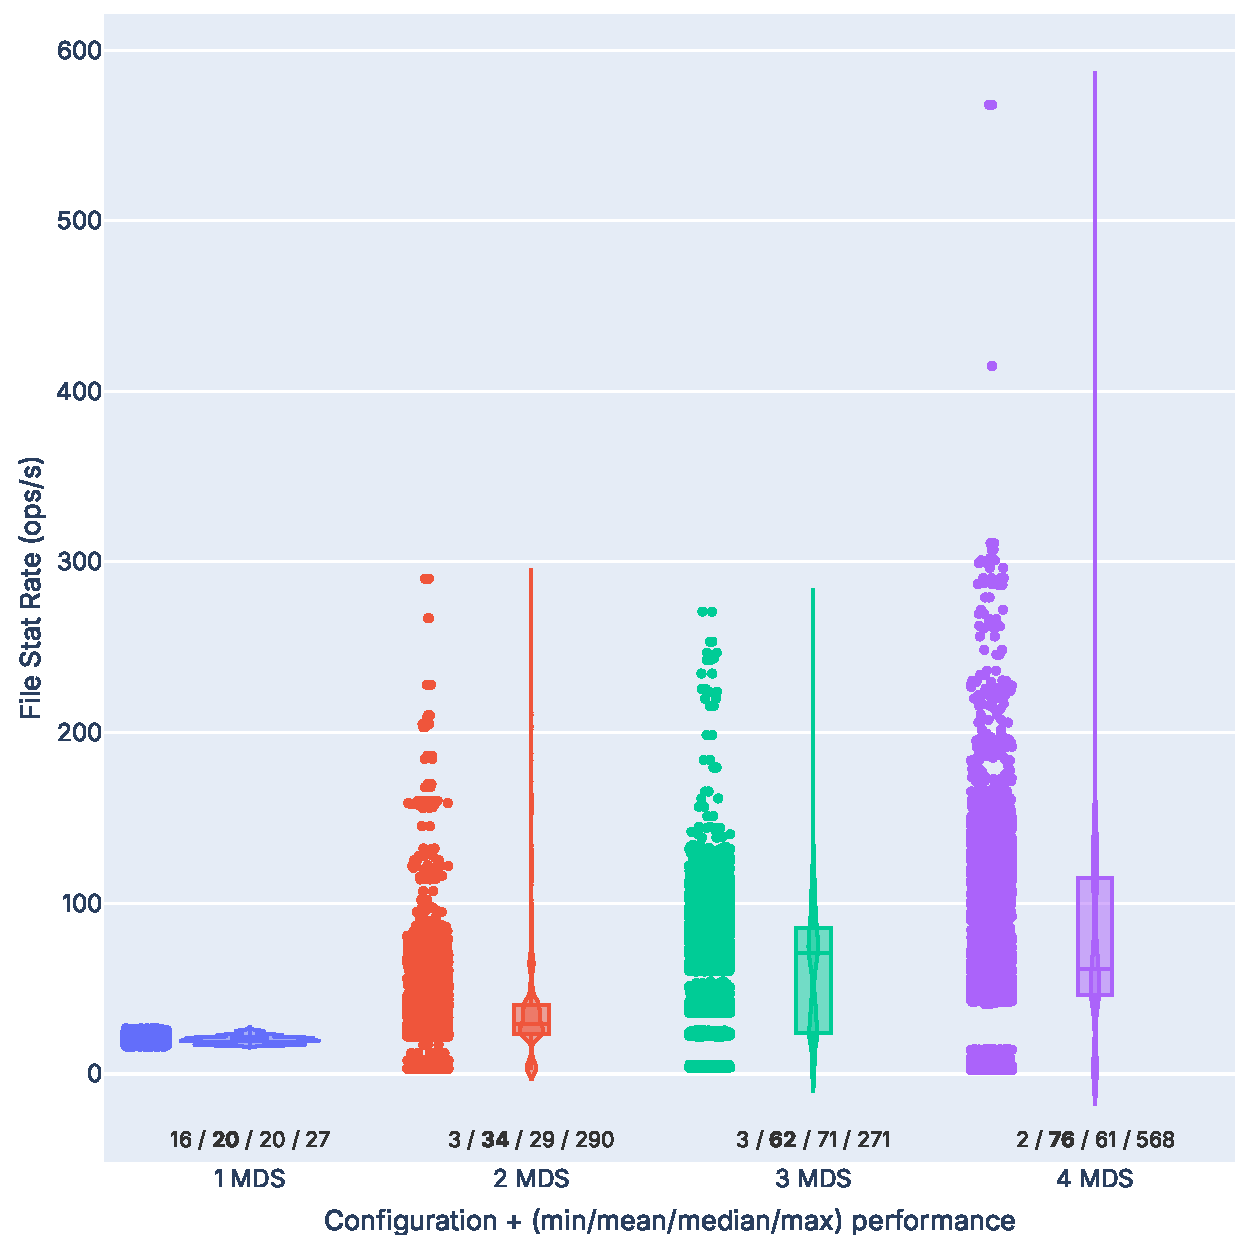
\includegraphics[width=\linewidth]{assets/perf_results/mdtest_violin_file_stat_8nodes_64tpn_mds_scaling.pdf}
    \caption[\acs{CephFS} MDS Scaling Performance -- File Stat Rate (8 nodes)]{Performance of the file stat operation per task with various numbers of active \acs{MDS} daemons with 512 total clients across 8 nodes, showing good scaling, albeit high performance variation.}
    \label{fig:mdtest-violin-file-stat-8n}
\end{figure}

\Cref{fig:mdtest-violin-file-stat-8n} shows the file stat rate observed at a per-task level. This specific run shows good performance scaling results; however, the large performance variance is likely due to the inconsistent distribution of client folders to \ac{MDS} daemons---clients which are on more lightly-loaded \ac{MDS} daemons are likely to have more performance available to them. Certain tasks in the 2- and 3-\acs{MDS} configurations seem to be severely performance-starved, which may be indicative of an overloaded \ac{MDS} daemon due to the inconsistent distribution.

\begin{figure}[H]
    \centering
    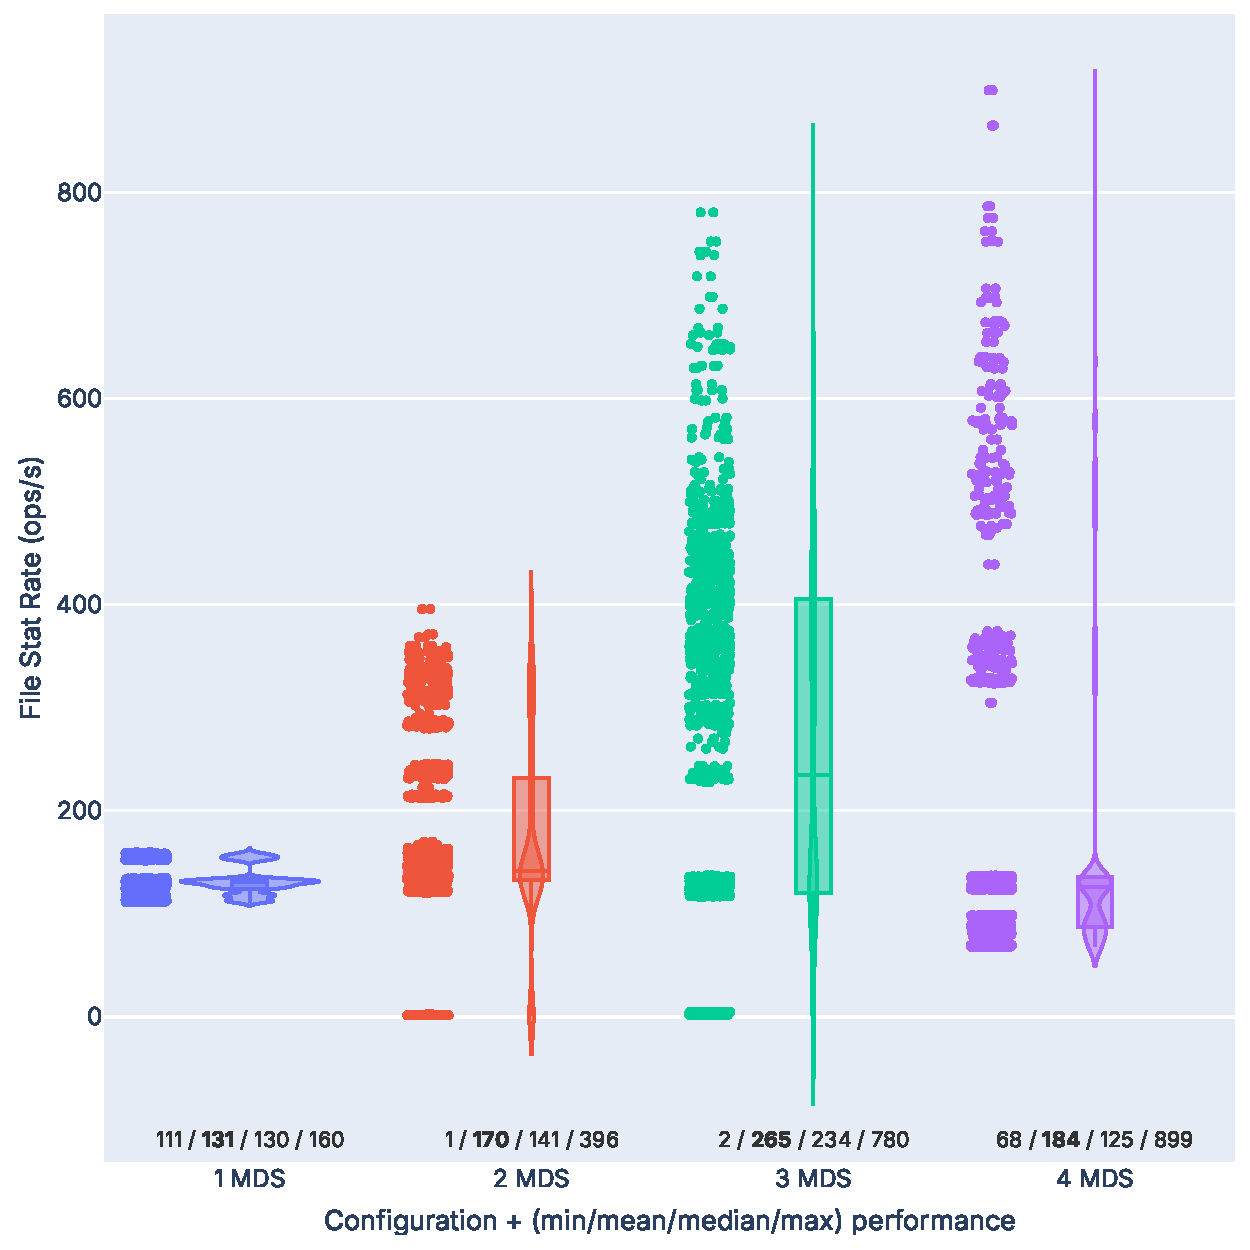
\includegraphics[width=1\linewidth]{assets/perf_results/mdtest_violin_file_stat_2nodes_64tpn_mds_scaling.pdf}
    \caption[\acs{CephFS} MDS Scaling Performance -- File Stat Rate (2 nodes)]{Performance of the file stat operation per task with various numbers of active \acs{MDS} daemons with 256 total clients across 2 nodes, showing inconsistent scaling results.}
    \label{fig:mdtest-violin-file-stat-2n}
\end{figure}

\Cref{fig:mdtest-violin-file-stat-2n} shows the file stat rate observed at a per-task level. In contrast to the 8-node results, these 2-node results show inconsistent performance scaling, with the 4-node configuration dropping below the performance of the 3-node configuration. The performance starvation of certain tasks is also observed in this run.

\subsubsection{Erasure-Coded Pools}

\begin{figure}[H]
    \centering
    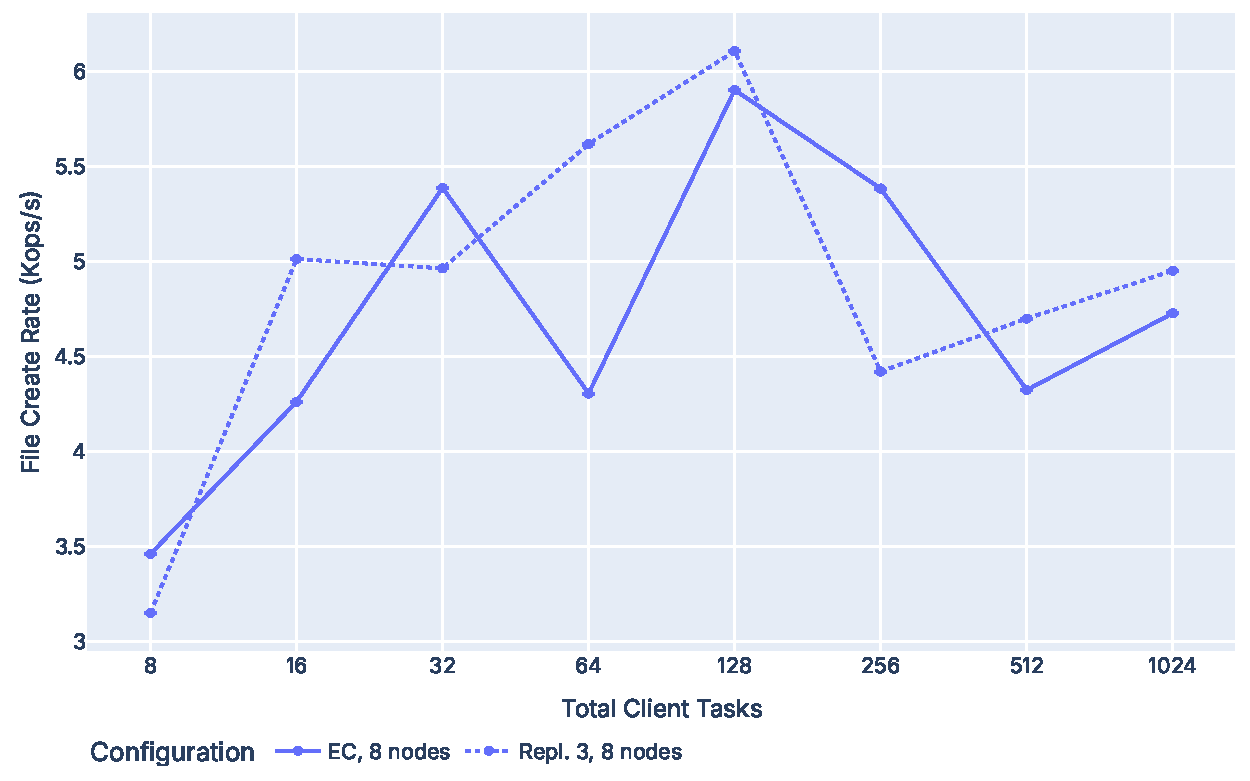
\includegraphics[width=0.9\linewidth]{assets/perf_results/mdtest_file_create_ec_vs_replicated.pdf}
    \caption[\acs{CephFS} Erasure-Coded File Creation Performance]{Performance of file creation operations on erasure-coded pools compared to replicated pools, showing similar performance ranges.}
    \label{fig:mdtest-file-create-ec-replicated}
\end{figure}

Erasure-coded pools demonstrated near-identical performance for metadata operations, such as file/folder creation and deletion. \Cref{fig:mdtest-file-create-ec-replicated} shows the file creation performance of an erasure-coded pool over a replicated pool for an 8-client-node benchmark run, showing similar performance. This is likely due to the fact that the \ac{MDS} metadata pool, which services such operations, uses the same replica-3 profile for both pool types---Ceph does not allow for the use of erasure-coded metadata pools. Therefore, identical performance is to be expected, and the gathered performance results support this.